% Crystal screening discussion slides: compile with latexmk -pdf idea-presentation.tex
% Self-contained references: no external bibliography or BibTeX step required.
\documentclass[10pt,aspectratio=169]{beamer}

\usetheme{Boadilla}
\usecolortheme{dove}
\usefonttheme{professionalfonts}
\setbeamertemplate{navigation symbols}{}
\setbeamersize{text margin left=7mm,text margin right=7mm}
\setbeamertemplate{footline}{%
  \leavevmode\hbox{% 
  \begin{beamercolorbox}[wd=.78\paperwidth,ht=2.6ex,dp=1ex,leftskip=1em]{author in head/foot}\insertshorttitle\end{beamercolorbox}%
  \begin{beamercolorbox}[wd=.22\paperwidth,ht=2.6ex,dp=1ex,rightskip=1em plus1fil]{date in head/foot}\insertframenumber\,/\,\inserttotalframenumber\end{beamercolorbox}}}

\usepackage{booktabs}
\usepackage{amsmath,amssymb}
\usepackage{tikz}
\usetikzlibrary{arrows.meta,positioning,fit,backgrounds,calc}
\usepackage{xcolor}

\definecolor{navy}{RGB}{22,51,86}
\definecolor{teal}{RGB}{0,121,140}
\definecolor{orange}{RGB}{207,111,35}
\definecolor{lightblue}{RGB}{230,240,247}
\setbeamercolor{structure}{fg=navy}
\setbeamercolor{frametitle}{fg=navy}
\setbeamercolor{title}{fg=navy}
\setbeamercolor{block title}{bg=navy,fg=white}
\setbeamercolor{block body}{bg=lightblue,fg=black}
\setbeamercolor{alertblock title}{bg=orange,fg=white}
\setbeamercolor{alertblock body}{bg=orange!12,fg=black}
\setbeamercolor{itemize item}{fg=teal}
\setbeamercolor{itemize subitem}{fg=teal}

\newcommand{\ehull}{E_{\mathrm{hull}}}
\newcommand{\embed}{\mathbf{h}}

\title[Graph-guided crystal screening]{Graph-Guided Reference Screening\\for Diffusion-Generated Crystals}
\subtitle{A proposal to improve Crys-JEPA's screening-and-refinement loop}
\author{}
\institute{}
\date{\today}

\begin{document}

\begin{frame}
  \titlepage
  \vfill
  \centering\scriptsize
  Motivation: Crys-JEPA \cite{liu2026crysjepa}, MatterGen \cite{MatterGen2025}, and MatterSim \cite{yang2024mattersim}
\end{frame}

\begin{frame}{Research objective}
\begin{block}{Question}
Can a \alert{chemistry-constrained graph over generated candidates and known reference phases} rank stable crystals better than Crys-JEPA's equal-weight embedding-distance heuristic?
\end{block}
\vspace{0.4em}
\begin{columns}[T]
\column{0.48\textwidth}
\textbf{Why it matters}
\begin{itemize}
  \item Diffusion models can generate many plausible periodic structures.
  \item Only a small fraction will be stable and novel after validation.
  \item Better screening can improve the data used for generator refinement.
\end{itemize}
\column{0.48\textwidth}
\textbf{Contribution hypothesis}
\begin{itemize}
  \item Crys-JEPA retrieves chemically related phases but aggregates them uniformly.
  \item A GNN can learn which phase relationships are useful for ranking.
  \item The main experiment keeps the encoder frozen for clean attribution.
\end{itemize}
\end{columns}
\end{frame}

\begin{frame}{Context: generation, relaxation, and refinement}
\centering
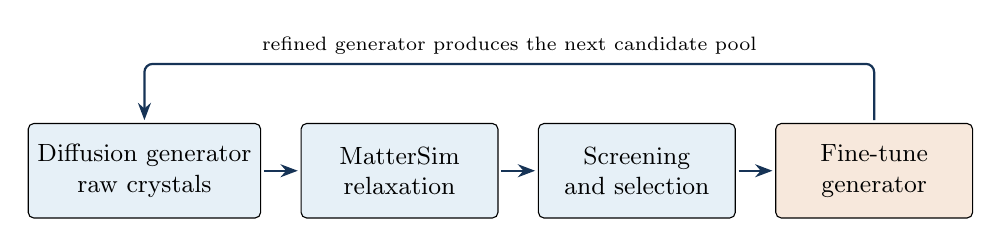
\begin{tikzpicture}[node distance=5mm and 5mm, every node/.style={font=\small,align=center}, box/.style={draw,rounded corners=2pt,minimum height=12mm,minimum width=25mm,fill=lightblue}, refinebox/.style={draw,rounded corners=2pt,minimum height=12mm,minimum width=25mm,fill=orange!16}, arr/.style={-{Stealth[length=2.2mm]},thick,navy}]
  \node[box] (gen) {Diffusion generator\\raw crystals};
  \node[box,right=of gen] (relax) {MatterSim\\relaxation};
  \node[box,right=of relax] (screen) {Screening\\and selection};
  \node[refinebox,right=of screen] (ft) {Fine-tune\\generator};
  \draw[arr,shorten <=1pt,shorten >=1pt] (gen.east)--(relax.west);
  \draw[arr,shorten <=1pt,shorten >=1pt] (relax.east)--(screen.west);
  \draw[arr,shorten <=1pt,shorten >=1pt] (screen.east)--(ft.west);
  \draw[arr,rounded corners=3pt,shorten <=1pt,shorten >=1pt]
    (ft.north) -- ++(0,0.75) -| (gen.north);
  \node[above,font=\scriptsize] at ($(gen.north)!0.5!(ft.north)+(0,0.75)$)
    {refined generator produces the next candidate pool};
\end{tikzpicture}
\vspace{0.8em}
\begin{itemize}
  \item \textbf{Relaxation} adjusts atomic coordinates and lattice parameters to reduce predicted energy and forces.
  \item MatterSim is a machine-learned force field: much cheaper than DFT, but not a substitute for final DFT validation \cite{yang2024mattersim}.
  \item Our intervention is the \alert{screening} box: improve what is selected for refinement.
\end{itemize}
\end{frame}

\begin{frame}{What MatterGen contributes}
\begin{columns}[T]
\column{0.56\textwidth}
\textbf{MatterGen} is a diffusion model that jointly denoises:
\begin{itemize}
  \item discrete atomic species;
  \item fractional coordinates on a periodic cell;
  \item lattice parameters.
\end{itemize}
It uses an equivariant, periodic atom-neighbour graph inside each crystal \cite{MatterGen2025}.
\vspace{0.4em}
\begin{alertblock}{Important distinction}
MatterGen's graph represents \textbf{atoms within one crystal}. This proposal builds a second graph whose nodes are \textbf{complete crystals}.
\end{alertblock}
\column{0.40\textwidth}
\centering
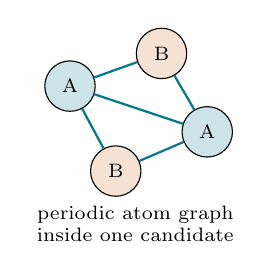
\begin{tikzpicture}[scale=.83, every node/.style={circle,draw,minimum size=6.4mm,font=\scriptsize}, edge/.style={teal,thick}]
  \node[fill=teal!20] (a) at (0,1.2) {A};
  \node[fill=orange!20] (b) at (1.4,1.7) {B};
  \node[fill=teal!20] (c) at (2.1,.5) {A};
  \node[fill=orange!20] (d) at (.7,-.1) {B};
  \draw[edge] (a)--(b)--(c)--(d)--(a);
  \draw[edge] (a)--(c);
  \node[draw=none,rectangle,font=\scriptsize,align=center] at (1,-.9) {periodic atom graph\\inside one candidate};
\end{tikzpicture}
\end{columns}
\end{frame}

\begin{frame}{Crys-JEPA screening and the proposed extension}
\begin{columns}[T]
\column{0.51\textwidth}
Crys-JEPA learns an energy-aware crystal embedding:
\[
  \text{crystal }x \longmapsto \embed_x .
\]
For a relaxed candidate $c$, it retrieves references $R(c)$ from the same chemical system and subsystems, and uses
\[
 D(c)=\frac{1}{|R(c)|}\sum_{r\in R(c)}\lVert\embed_c-\embed_r\rVert_2^2.
\]
Smaller distance $D(c)$ means a more promising candidate \cite{liu2026crysjepa}.
\column{0.45\textwidth}
\begin{alertblock}{Limitation}
References form an \textbf{unstructured, equal-weight set}.
\begin{itemize}
  \item All retrieved phases contribute equally.
  \item Reference--reference relationships are discarded.
  \item The score can be sensitive to redundant or weakly relevant references.
\end{itemize}
\end{alertblock}
\end{columns}
\end{frame}

\begin{frame}{Proposed idea: a local chemistry-aware reference graph}
\centering
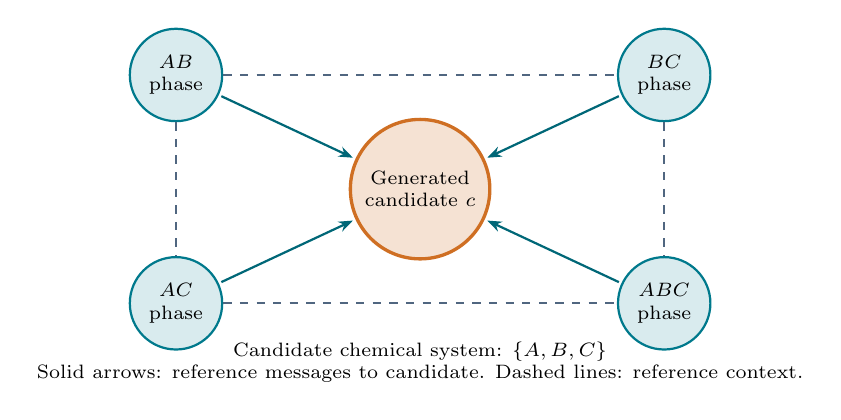
\begin{tikzpicture}[node distance=12mm, every node/.style={align=center,font=\scriptsize}, cand/.style={circle,draw=orange,very thick,fill=orange!20,minimum size=16mm}, ref/.style={circle,draw=teal,thick,fill=teal!15,minimum size=11mm}, edge/.style={-{Stealth[length=1.8mm]},thick,teal!85!black,shorten <=1pt,shorten >=1pt}, sim/.style={thick,dashed,navy!75}]
  \node[cand] (q) at (0,0) {Generated\\candidate $c$};
  \node[ref] (ab) at (-3.1,1.45) {$AB$\\phase};
  \node[ref] (ac) at (-3.1,-1.45) {$AC$\\phase};
  \node[ref] (bc) at (3.1,1.45) {$BC$\\phase};
  \node[ref] (abc) at (3.1,-1.45) {$ABC$\\phase};
  \node[draw=none,rectangle,font=\scriptsize,align=center] (chem) at (0,-2.2) {Candidate chemical system: $\{A,B,C\}$\\Solid arrows: reference messages to candidate. Dashed lines: reference context.};
  \draw[edge] (ab)--(q); \draw[edge] (ac)--(q); \draw[edge] (bc)--(q); \draw[edge] (abc)--(q);
  \draw[sim] (ab)--(ac); \draw[sim] (ab)--(bc); \draw[sim] (bc)--(abc); \draw[sim] (ac)--(abc);
\end{tikzpicture}
\vspace{0.25em}
\begin{itemize}
  \item \textbf{Nodes:} complete relaxed generated crystals and known reference phases.
  \item \textbf{Edges:} first enforce chemical validity; then retain $k$ nearest neighbours in frozen Crys-JEPA embedding space.
  \item \textbf{Edge features:} embedding distance, relation type (exact system / subsystem), and composition similarity.
\end{itemize}
\end{frame}

\begin{frame}{Model: learn relevance, not merely proximity}
\begin{columns}[T]
\column{0.56\textwidth}
For candidate $c$, construct its allowable reference pool only from training-side phases:
\[
R_{\mathrm{valid}}(c)=\{r:\;\mathrm{elements}(r)\subseteq\mathrm{elements}(c)\}.
\]
Build a small local graph with $k\in\{8,16,32\}$ retrieved references and apply an edge-aware GNN:
\[
\widehat{p}_{\mathrm{stable}}(c)=\mathrm{GNN}(G_c).
\]
\begin{itemize}
  \item Start with two-layer GraphSAGE or graph attention.
  \item Retain a direct candidate-feature path to avoid over-smoothing.
  \item Predict stability class or a ranking score for low $\ehull$.
\end{itemize}
\column{0.40\textwidth}
\begin{block}{Why a graph?}
The model can learn that some phase relations are informative while others are not, and can use reference--reference context.
\end{block}
\begin{alertblock}{Controlled comparison}
Freeze Crys-JEPA embeddings to isolate the effect of graph aggregation under matched supervision.
\end{alertblock}
\end{columns}
\end{frame}

\begin{frame}{Experimental protocol: make the claim falsifiable}
\begin{columns}[T]
\column{0.49\textwidth}
\textbf{Data and splits}
\begin{itemize}
  \item Use generated, MatterSim-relaxed candidate structures with a fixed stability-label protocol.
  \item Build all references from the training split only.
  \item Hold out related relaxation snapshots together.
  \item Add formula- or prototype-held-out evaluation for transfer.
\end{itemize}
\column{0.49\textwidth}
\textbf{Matched baselines}
\begin{enumerate}
  \item Original Crys-JEPA average-distance score.
  \item Nearest-neighbour and inverse-distance scores.
  \item Candidate-only MLP on the same frozen embedding.
  \item Set model seeing the same retrieved references but no graph topology.
  \item Proposed GNN.
\end{enumerate}
\end{columns}
\vspace{0.5em}
\begin{alertblock}{Interpretation rule}
If the set model matches the GNN, the gain comes from retrieval rather than graph structure.
\end{alertblock}
\end{frame}

\begin{frame}{Evaluation and success criteria}
\begin{columns}[T]
\column{0.49\textwidth}
\textbf{Primary metrics}
\begin{itemize}
  \item Precision@top 10\% and top 20\% for stable / near-hull candidates.
  \item Recall of low-$\ehull$ candidates.
  \item AUROC or ranking metrics as secondary measures.
  \item Screening and graph-construction runtime.
\end{itemize}
\column{0.49\textwidth}
\textbf{Robustness tests}
\begin{itemize}
  \item Vary $k$ and relation types.
  \item Remove irrelevant neighbours.
  \item Duplicate a reference entry: a robust model should not change materially.
  \item Test transfer to generated candidates and unfamiliar prototypes.
\end{itemize}
\end{columns}
\vspace{0.6em}
\begin{block}{Success}
The GNN consistently beats both the original score \emph{and} an equally informed set baseline on held-out and generated candidates.
\end{block}
\end{frame}

\begin{frame}{References}
\small
\setbeamertemplate{bibliography item}[text]
\setbeamerfont{bibliography entry author}{size=\small}
\setbeamerfont{bibliography entry title}{size=\small}
\setbeamerfont{bibliography entry location}{size=\footnotesize}
\setbeamerfont{bibliography entry note}{size=\footnotesize}
\begin{thebibliography}{3}
\bibitem{liu2026crysjepa}
Nian Liu et al.
\newblock Crys-JEPA: Accelerating Crystal Discovery via Embedding Screening and Generative Refinement.
\newblock arXiv preprint, 2026.
\newblock \href{https://arxiv.org/abs/2605.14759}{arXiv:2605.14759}
\vspace{0.5em}
\bibitem{MatterGen2025}
Claudio Zeni et al.
\newblock A generative model for inorganic materials design.
\newblock \emph{Nature}, 2025.
\newblock \href{https://doi.org/10.1038/s41586-025-08628-5}{doi:10.1038/s41586-025-08628-5}
\vspace{0.5em}
\bibitem{yang2024mattersim}
Han Yang et al.
\newblock MatterSim: A Deep Learning Atomistic Model Across Elements, Temperatures and Pressures.
\newblock arXiv preprint arXiv:2405.04967, 2024.
\newblock \href{https://arxiv.org/abs/2405.04967}{arXiv:2405.04967}
\end{thebibliography}
\end{frame}

\end{document}
